\documentclass[conference]{IEEEtran}
% IEEEtran conference template (Michael Shell). Build: latexmk -pdf main.tex
\IEEEoverridecommandlockouts

\usepackage{cite}
\usepackage{amsmath,amssymb,amsfonts}
\usepackage{algorithm}
\usepackage{algorithmic}
\usepackage{graphicx}
\usepackage{textcomp}
\usepackage{xcolor}
\usepackage{booktabs}
\usepackage{array}
\usepackage{url}
\usepackage{tikz}
\usetikzlibrary{arrows.meta,positioning,calc,fit}

% Affiliation of all four authors: replace before submission.
\newcommand{\affil}{[Department], [Institution]\\{}[City], [Country]}

\renewcommand{\algorithmicrequire}{\textbf{Input:}}
\renewcommand{\algorithmicensure}{\textbf{Output:}}

\begin{document}

\title{Agentic AI-Based Model Regeneration\\ Framework for O-RAN}

\author{%
\IEEEauthorblockN{Ramanujam P}
\IEEEauthorblockA{\affil\\ pramanujam68@gmail.com}
\and
\IEEEauthorblockN{Nitesh N D}
\IEEEauthorblockA{\affil\\ niteshdwaraka@gmail.com}
\and
\IEEEauthorblockN{Tamilselvan R}
\IEEEauthorblockA{\affil\\ tamilraj1402@gmail.com}
\and
\IEEEauthorblockN{Bhuvaneshwar T S}
\IEEEauthorblockA{\affil\\ bhuvaneshwarts1@gmail.com}}

\maketitle

\begin{abstract}
AI/ML models deployed in the Open Radio Access Network (O-RAN) degrade as traffic, load, and
radio conditions evolve, and current MLOps workflows leave the choice of remedy to human
operators. This paper presents an Agentic AI-based model regeneration framework that acts on a
reported degradation and decides, without human intervention, how the deployed model should be
readapted. After quantifying the shift with the Kolmogorov--Smirnov test and the Population
Stability Index (PSI), the framework attempts a \emph{similar model exchange} that re-scores every
registered version on held-out current data and promotes one that measurably beats the deployed
model. Otherwise a Decision Engine, combining hard constraints with an optional large language
model (LLM) agent that calls read-only evidence tools, selects Finetune, Regenerate, Rollback, or
No Action, and an engine selection stage runs the action with a native engine or, only if none
exists, with LLM-written code that is checked against an abstract-syntax-tree whitelist and
sandboxed. A paired-bootstrap gate admits a candidate only when its improvement is established.
On eight controlled drift scenarios, remediation reduces held-out RMSE by 62.5--97.5\,\% under
concept drift but changes it by less than 1\,\% under pure covariate shift although PSI reaches
15.6, so PSI is a sound severity measure but an unsafe trigger. The gate rejects a candidate whose
95\,\% interval straddles zero although its point estimate exceeds in magnitude that of an
accepted candidate.
\end{abstract}

\begin{IEEEkeywords}
Agentic AI, O-RAN, MLOps, model lifecycle management, concept drift, population stability
index, bootstrap, large language model.
\end{IEEEkeywords}

\section{Introduction}
The Open Radio Access Network (O-RAN) enables intelligent, programmable RAN operation through
software-defined control and AI/ML applications hosted in the RAN Intelligent Controllers
\cite{polese2023understanding}. Models that run continuously in such an environment degrade as
network behaviour, workload, and operating conditions change: the input distribution $P(X)$, the
input--output relationship $P(y\mid X)$, or both shift over time \cite{ditzler2015learning}.

Existing MLOps workflows for O-RAN monitor models and retrain them through hand-built pipelines
\cite{li2022rlops,parraullauri2025reason}, but the decision of \emph{how} to remediate a degraded
production model, by reusing an earlier version, fine-tuning, retraining from scratch, rolling
back, or doing nothing, remains with a human operator. This paper addresses that decision. Its
contributions are:
\begin{itemize}
\item a closed-loop readaptation pipeline that measures the shift, attempts a similar model
exchange from the version registry, and otherwise lets a constraint-bounded Decision Engine
choose among Finetune, Regenerate, Rollback, and No Action;
\item an engine selection stage that falls back to LLM-written adaptation code only when no
native engine exists, with an AST whitelist, sandboxed execution, and a bounded
write--check--run--fix loop;
\item a paired-bootstrap deployment gate that admits a candidate only if its improvement is
established at 95\,\% confidence; and
\item a reproducible evaluation on eight controlled drift scenarios, showing why PSI belongs
after a degradation report as a severity measure rather than before it as a trigger.
\end{itemize}

\section{Related Work}
Table~\ref{tab:lit} summarises the fifteen works reviewed, in four groups.

\emph{Agentic and closed-loop control.} Mekrache \textit{et al.}~\cite{mekrache2024intent}
place an LLM at the centre of the intent life cycle on a 5G testbed, but do not decide when a
deployed model must be retrained. DRL xApps run in O-RAN control loops~\cite{bonati2021intelligence},
and ColO-RAN~\cite{polese2023coloran} shows that they need online retraining once deployed,
leaving when and how to the designer.

\emph{Lifecycle management.} RLOps~\cite{li2022rlops} lays out an MLOps life cycle for
learning-based O-RAN control without automating the choice of action.
REASON~\cite{parraullauri2025reason} adds AI orchestration, monitoring, and a digital-twin check
before deployment, but its pipelines are not driven by a remediation decision.

\emph{Conflict and intent.} Adamczyk and Kliks~\cite{adamczyk2023conflict} detect direct,
indirect, and implicit xApp conflicts in the near-RT RIC, and QACM~\cite{wadud2024qacm}
mitigates them with QoS awareness; surveys cover LLMs for telecommunications~\cite{zhou2025llm}
and intent-based networking~\cite{leivadeas2023survey}. None manages a model's lifecycle after
it degrades.

\emph{Twins, orchestration, and drift.} Digital twins test changes off the live
network~\cite{masaracchia2023digital} and gain a 6G reference
architecture~\cite{zakihindi2026reference}; a DRL traffic-steering xApp raises throughput by
50\,\%~\cite{lacava2024programmable}; OrchestRAN~\cite{doro2022orchestran} decides which models
run where; and a drift module for the 5G core detects drift and retrains~\cite{manias2022model}.
The remediation decision rests on the concept-drift literature: Ditzler
\textit{et al.}~\cite{ditzler2015learning} separate covariate shift, where $P(X)$ changes, from
real concept drift, where $P(y\mid X)$ changes, and Lu \textit{et al.}~\cite{lu2019learning}
survey detection and adaptation. Neither prescribes which remedy fits a given shift signature,
which is the decision the Decision Engine makes.

\begin{table*}[t]
\centering
\caption{Summary of the Reviewed Literature}
\label{tab:lit}
\scriptsize
\setlength{\tabcolsep}{3pt}
\newcolumntype{L}[1]{>{\raggedright\arraybackslash}p{#1}}
\begin{tabular}{@{}r L{3.5cm} L{3.7cm} L{2.9cm} L{6.6cm}@{}}
\toprule
No. & Work & Venue, year & Category & Key points and gap with respect to this work\\
\midrule
1 & LLM-centric intent management~\cite{mekrache2024intent} & IEEE Network, 2024 & Agentic; intent; LLM & LLM translates and assures intents; no retraining decision\\
2 & Intelligence in O-RAN~\cite{bonati2021intelligence} & IEEE Commun. Mag., 2021 & Closed-loop AI control & DRL xApps in RIC control loops; model upkeep left open\\
3 & ColO-RAN~\cite{polese2023coloran} & IEEE Trans. Mobile Comput., 2023 & ML xApp pipeline & Deployed agents need online retraining; when and how not decided\\
4 & RLOps~\cite{li2022rlops} & IEEE Access, 2022 & ML life cycle (MLOps) & Specify, develop, serve, monitor, retrain; action choice is manual\\
5 & REASON~\cite{parraullauri2025reason} & IEEE Wireless Commun., 2025 & Trustworthy AI lifecycle & Orchestration, monitoring, twin check before deployment; no remedy choice\\
6 & Near-RT RIC conflicts~\cite{adamczyk2023conflict} & IEEE Commun. Mag., 2023 & xApp conflict detection & Direct, indirect, implicit conflicts; no model lifecycle\\
7 & LLM for telecommunications~\cite{zhou2025llm} & IEEE Commun. Surveys Tuts., 2025 & LLM survey & Generation, classification, optimisation; no model readaptation\\
8 & Intent-based networking~\cite{leivadeas2023survey} & IEEE Commun. Surveys Tuts., 2023 & Intent-based networking & Translation, activation, assurance; no ML lifecycle\\
9 & QACM~\cite{wadud2024qacm} & IEEE Trans. Green Commun. Netw., 2024 & xApp conflict mitigation & Sets conflicting parameters so most xApps meet QoS\\
10 & Digital twin for Open RAN~\cite{masaracchia2023digital} & IEEE Commun. Mag., 2023 & Network digital twin & Twin tests changes off the live network; use cases\\
11 & Traffic-steering xApp~\cite{lacava2024programmable} & IEEE Trans. Mobile Comput., 2024 & DRL handover control & 50\,\% higher throughput; trained once, no retraining policy\\
12 & Reference NDT architecture~\cite{zakihindi2026reference} & IEEE Open J. Commun. Soc., 2026 & Digital twin architecture & AI workflows, simulation, data, orchestration, twin lifecycle\\
13 & OrchestRAN~\cite{doro2022orchestran} & IEEE INFOCOM, 2022 & Model orchestration & Chooses which models run where; no degradation-driven update\\
14 & Model drift in 5G core~\cite{manias2022model} & IEEE MeditCom, 2022 & Drift detection and adaptation & Detects drift and retrains; a single remedy, no choice\\
15 & Understanding O-RAN~\cite{polese2023understanding} & IEEE Commun. Surveys Tuts., 2023 & O-RAN architecture & Architecture, interfaces, algorithms, security, challenges\\
\bottomrule
\end{tabular}
\end{table*}

\section{Research Gaps}
The reviewed works leave three gaps that this framework addresses.
\begin{itemize}
\item \emph{G1 (Autonomous readaptation):} when to retrain and which action to take remain
open~\cite{mekrache2024intent,bonati2021intelligence,polese2023coloran}, and life cycles stop at
hand-built pipelines~\cite{li2022rlops,parraullauri2025reason}. An autonomous readapter should
first try to reuse an earlier model version that already fits the current data.
\item \emph{G2 (Remediation logic):} a degradation signal is uncertain---xApp conflicts can
degrade a model that is still correct~\cite{adamczyk2023conflict}---and drift
modules~\cite{manias2022model} retrain without choosing a remedy. Missing is a Finetune,
Regenerate, Rollback, or No Action decision that acts on a reported degradation and uses the
measured shift only as severity.
\item \emph{G3 (Verified promotion):} trust gates, twins, and model
orchestration~\cite{parraullauri2025reason,zakihindi2026reference,doro2022orchestran} decide
what is deployed, but none states a statistical rule that rejects a candidate whose improvement
is not established.
\end{itemize}

\section{Proposed Framework}

\subsection{Pipeline Overview}
Fig.~\ref{fig:arch} and Algorithm~\ref{alg:pipeline} give the pipeline end to end. The framework
does not detect drift itself: an external monitor, or one of the framework's declarative event
mappers, reports a degradation for a model and names the current data. The Intake Agent validates
the report, checks that the model exists in the MLflow registry, and enqueues a job; a worker
leases it (a crashed worker's job is picked up again) and executes the stages below, and every
transition of the sixteen-state job life cycle is recorded with a timestamp, actor, and reason.

\begin{figure*}[t]
\centering
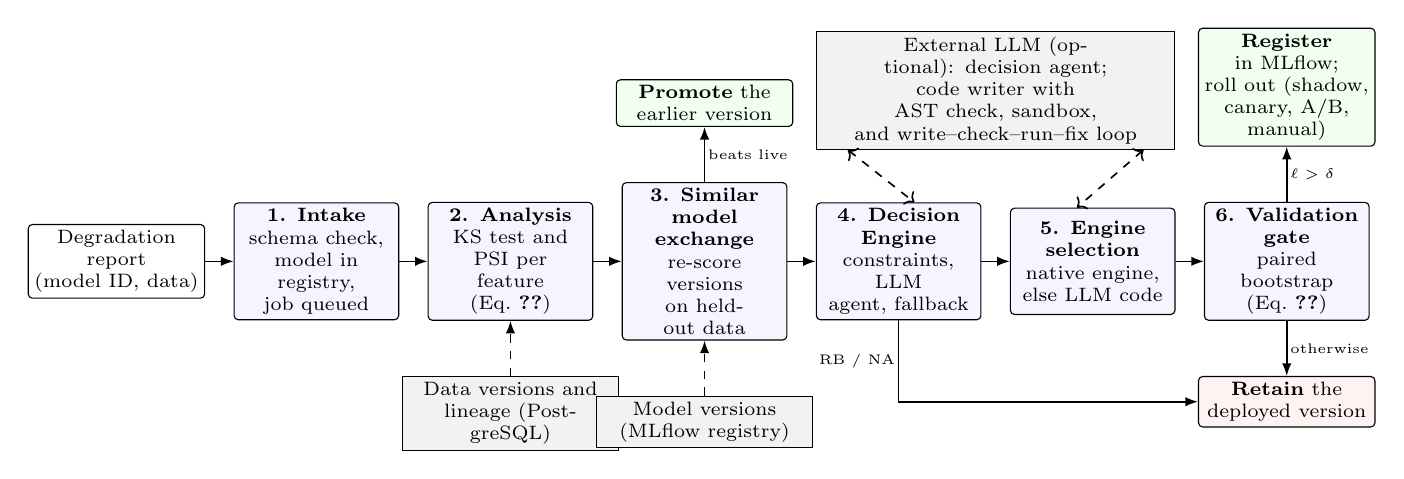
\begin{tikzpicture}[
  font=\scriptsize, node distance=3.2mm and 3.6mm,
  stage/.style={draw, rounded corners=1.5pt, align=center, minimum height=13.5mm,
    text width=19.5mm, inner sep=2pt, fill=blue!4},
  store/.style={draw, align=center, text width=26mm, inner sep=2pt, fill=gray!10},
  term/.style={draw, rounded corners=1.5pt, align=center, text width=21mm, inner sep=2pt},
  arr/.style={-{Latex[length=1.6mm]}, semithick},
  lab/.style={font=\tiny, inner sep=1pt}]
\node[term] (rep) {Degradation report\\ (model ID, data)};
\node[stage, right=of rep] (intake) {\textbf{1. Intake}\\ schema check,\\ model in registry,\\ job queued};
\node[stage, right=of intake] (an) {\textbf{2. Analysis}\\ KS test and PSI per\\ feature (Eq.~\ref{eq:psi})};
\node[stage, right=of an] (sme) {\textbf{3. Similar model}\\ \textbf{exchange}\\ re-score versions\\ on held-out data};
\node[stage, right=of sme] (dec) {\textbf{4. Decision}\\ \textbf{Engine}\\ constraints, LLM\\ agent, fallback};
\node[stage, right=of dec] (eng) {\textbf{5. Engine}\\ \textbf{selection}\\ native engine,\\ else LLM code};
\node[stage, right=of eng] (gate) {\textbf{6. Validation}\\ \textbf{gate}\\ paired bootstrap\\ (Eq.~\ref{eq:gate})};
\node[term, above=7mm of gate, fill=green!6] (reg) {\textbf{Register} in MLflow;\\ roll out (shadow,\\ canary, A/B, manual)};
\node[term, below=7mm of gate, fill=red!5] (keep) {\textbf{Retain} the\\ deployed version};
\node[term, above=7mm of sme, fill=green!6] (promote) {\textbf{Promote} the\\ earlier version};
\node[store, below=7mm of an] (pg) {Data versions and\\ lineage (PostgreSQL)};
\node[store, below=7mm of sme] (ml) {Model versions\\ (MLflow registry)};
\coordinate (decengtop) at ($(dec.north)!0.5!(eng.north)$);
\node[store, above=7mm of decengtop, anchor=south, text width=44mm] (llm) {External LLM (optional): decision agent;\\ code writer with AST check, sandbox,\\ and write--check--run--fix loop};
\draw[arr] (rep) -- (intake);
\draw[arr] (intake) -- (an);
\draw[arr] (an) -- (sme);
\draw[arr] (sme) -- (dec);
\draw[arr] (dec) -- (eng);
\draw[arr] (eng) -- (gate);
\draw[arr] (gate) -- node[lab, right]{$\ell>\delta$} (reg);
\draw[arr] (gate) -- node[lab, right]{otherwise} (keep);
\draw[arr] (sme) -- node[lab, right]{beats live} (promote);
\draw[arr] (dec.south) |- node[lab, pos=0.25, left]{RB / NA} (keep.west);
\draw[arr, dashed] (pg) -- (an);
\draw[arr, dashed] (ml) -- (sme);
\draw[arr, dashed, <->] (llm.south west) ++(4mm,0) -- ($(dec.north)+(2mm,0)$);
\draw[arr, dashed, <->] (llm.south east) ++(-4mm,0) -- ($(eng.north)+(-2mm,0)$);
\end{tikzpicture}
\caption{Architecture of the regeneration pipeline. Solid arrows: control flow; dashed arrows:
data and optional LLM calls. The exchange hands over to the Decision Engine only when no registered
version beats the deployed one, and only Finetune (FT) and Regenerate (RG) reach engine selection;
Rollback (RB) and No Action (NA) retain the deployed version.}
\label{fig:arch}
\end{figure*}

\begin{algorithm}[t]
\caption{Readaptation pipeline for one degradation report}
\label{alg:pipeline}
\begin{algorithmic}[1]
\REQUIRE model ID, reference to the current data $D_c$
\STATE Validate the report; reject it if the schema check fails or the model is unknown
\STATE Load the training data $D_r$ of the deployed version $M_t$ and the current data $D_c$
\STATE Compute the KS $p$-value and PSI (Eq.~\ref{eq:psi}) of every feature
\STATE Hold out the newest fraction $H$ of $D_c$ (never trained on)
\STATE Score every registered version on $H$ (similar model exchange)
\IF{a compatible version beats $M_t$ by the reuse margin}
  \STATE Promote that version; \textbf{return}
\ENDIF
\STATE $a \leftarrow$ Decision Engine (Eqs.~\ref{eq:actions}--\ref{eq:rule})
\IF{$a \in \{\text{Rollback}, \text{No Action}\}$}
  \STATE Retain $M_t$; \textbf{return}
\ENDIF
\STATE $M_{\text{cand}} \leftarrow$ native engine of the model type for $a$; if none, a full
retrain when supported, else LLM-written code (AST check, sandbox, bounded repair loop)
\IF{the gate of Eq.~\ref{eq:gate} accepts $M_{\text{cand}}$ on $H$}
  \STATE Register $M_{\text{cand}}$ and roll it out with the configured delivery strategy
\ELSE
  \STATE Retain $M_t$
\ENDIF
\end{algorithmic}
\end{algorithm}

\subsection{Shift Analysis}
The current data and the deployed version's training data are retrieved from versioned,
content-hashed data versions whose lineage links each model version to the exact rows it was
trained on. For every numeric feature the framework computes the two-sample
Kolmogorov--Smirnov test and the PSI of Eq.~\eqref{eq:psi}. These statistics are evidence for
the later stages; they do not by themselves start or stop remediation.

\subsection{Similar Model Exchange}
Rather than a separate catalog of models and environments, the version registry itself is
searched. Up to ten of the newest registered versions, and the deployed one, are re-scored on
the held-out slice $H$ of the current data. A version is compatible when its artifact passes its
checksum, loads, is of the same estimator kind, and finds all its features in the data. A
compatible, non-deployed version that lowers the deployed version's RMSE by at least 5\,\% (or
raises a classifier's accuracy by at least 0.02) is promoted directly, with no training and no
candidate gate. Otherwise the scores are handed to the Decision Engine.

\subsection{Decision Engine}
The Decision Engine chooses among the actions of Eq.~\eqref{eq:actions}. Hard constraints come
first and cannot be overruled: too few current rows or an insufficient sample stop the job as
\emph{insufficient information}; a framework without an adaptation engine stops it as \emph{no
compatible strategy}; a maximum feature PSI of at least $\tau = 0.5$ rules out Finetune, so a
severe shift is always regenerated; and Rollback requires recent performance data and a
compatible earlier version. When an LLM is configured, it chooses among the remaining actions,
either from a single structured prompt or, if enabled, as an agent that calls read-only tools
(shift summary, per-feature statistics, version scores, constraints, per-action cost and
expected-gain estimates) for a bounded number of steps before it submits. An answer outside the
feasible set, a malformed answer, an unreachable LLM, or an exhausted step budget falls back to
the deterministic preference order of Eq.~\eqref{eq:rule}. Every decision is stored with its
evidence, thresholds, source, and, for the agent, its full tool trace. A Rollback or No Action
decision trains nothing and keeps the deployed version; re-promoting an earlier version is the
job of the similar model exchange, which acts only when that version measurably wins.

\subsection{Engine Selection}
Finetune continues training a copy of the deployed model from its current state: through
\texttt{partial\_fit} for incremental scikit-learn estimators and by continued gradient descent
from the current weights for PyTorch modules. Regenerate refits the same estimator
configuration from scratch. Each model family is a registered model-type plugin (scikit-learn,
XGBoost, LightGBM, CatBoost, PyTorch, PyTorch sequence models, Keras, ONNX, and statsmodels), so
a new family is added by registration rather than by changing the pipeline. If the plugin has no
engine for the chosen action, a Finetune falls back to a full retrain when the model supports
it; only otherwise, and only when an LLM is configured, an external LLM writes an
\texttt{adapt()} function. That code is rejected unless it passes an AST whitelist of imports,
built-ins, and attributes, and it runs in a sandboxed subprocess or container with time and
memory limits; only the fitted model crosses back. Optionally, a rejected or failing attempt is
returned to the LLM with the scan violations or the sandbox traceback for a bounded number of
repair attempts. If every path fails, the job ends with a typed error and the deployed version
is retained.

\subsection{Validation, Registration, and Delivery}
The candidate is scored against the deployed model on the same held-out slice $H$ by the gate of
Eq.~\eqref{eq:gate}, together with configurable guardrails on data slices, calibration,
latency, and model size. An accepted candidate is registered as a new MLflow version with the data version it was
trained on, and rolled out by the configured delivery strategy (shadow, canary, blue--green, A/B,
or manual approval) with automatic rollback on a breached health rule.

\section{Mathematical Formulation}

\subsection{Shift Severity}
For a feature with reference sample (training data) and current sample, the PSI over $B$ bins is
\begin{equation}
\mathrm{PSI} = \sum_{i=1}^{B} (P_i - Q_i)\,\ln\frac{P_i}{Q_i},
\label{eq:psi}
\end{equation}
where $P_i$ and $Q_i$ are the reference and current proportions in bin $i$. The bins follow
Sturges' rule over the pooled sample, and an empty bin is assigned a proportion of $10^{-4}$, so
a shift that moves the current data outside the reference range yields large values (above 15 in
Section~\ref{sec:results}). The pipeline uses $\mathrm{PSI}_{\max}$, the maximum over features.

\subsection{Readaptation Policy}
The action set is
\begin{equation}
\mathcal{A} = \{\text{Finetune}, \text{Regenerate}, \text{Rollback}, \text{No Action}\}.
\label{eq:actions}
\end{equation}
Let $\mathcal{R}(c)\subseteq\mathcal{A}$ be the actions ruled out by the hard constraints $c$,
including Finetune whenever $\mathrm{PSI}_{\max} \ge \tau$. With the feasible set
$\mathcal{F} = \mathcal{A}\setminus\mathcal{R}(c)$, the selected action is
\begin{equation}
a^{*} =
\begin{cases}
a_{\mathrm{LLM}}, & \text{if } a_{\mathrm{LLM}} \in \mathcal{F},\\
\text{first of } \mathcal{F} \text{ in } (\text{FT}, \text{RG}, \text{RB}, \text{NA}), & \text{otherwise},
\end{cases}
\label{eq:rule}
\end{equation}
where $a_{\mathrm{LLM}}$ is the LLM's answer, if any, and the fallback prefers the least costly
feasible action.

\subsection{Deployment Gate Criterion}
A candidate produced by Finetune or Regenerate is admitted only if it is demonstrably superior to
the incumbent, not merely different from it. Let $m$ be the quality metric oriented so that larger
is better, and let $H$ be the time-ordered held-out slice on which neither model was trained.
Drawing $B'$ paired bootstrap resamples~\cite{zoubir1998bootstrap}, both models are scored on the
same resampled rows, and the improvement $\Delta = m(M_{\text{cand}}) - m(M_t)$ receives a
two-sided percentile interval $[\ell, u]$ at confidence $1-\alpha$. The candidate is deployed
when
\begin{equation}
\ell > \delta, \qquad \delta = 0,\; 1-\alpha = 0.95,\; B' = 1000.
\label{eq:gate}
\end{equation}
Because the criterion depends on the lower bound $\ell$ rather than on the point estimate
$\Delta$, any candidate whose interval contains zero is rejected.

\section{Implementation}
The framework comprises 33\,528 lines of Python in 186 modules, with 961 automated tests. The
service exposes 39 REST endpoints covering intake, job control, model and data versions, gate
decisions, and rollouts. Intake only validates and enqueues; separate workers lease jobs from a
durable queue (database, Celery, RQ, or Kubernetes jobs). The data versions and the job, audit,
and gate records are kept in PostgreSQL (SQLite for development), and model artifacts in MLflow.
The LLM is reached through one port with interchangeable providers (Google Gemini by default,
Anthropic, or any OpenAI-compatible endpoint, including a self-hosted one); every call is
recorded with its versioned prompt, tokens, and cost, guarded by retries, a circuit breaker, and
a budget, and without a configured key every decision takes the deterministic path.

\section{Experimental Setup}
The evaluation uses synthetic cell-level KPIs with three features, PRB utilisation
(\texttt{prb\_util}), CQI (\texttt{cqi}), and RSRP (\texttt{rsrp}), scaled to about $[0,1]$,
against throughput $y = \beta\,\texttt{prb\_util} + 0.8\,\texttt{cqi} + 0.5\,\texttt{rsrp} +
\varepsilon$ with $\varepsilon \sim \mathcal{N}(0, 0.1^2)$. A baseline window of 600 records
represents the environment of the deployed model $M_t$, an SGD linear regressor. Eight drifted
windows of 600 records vary two generator parameters independently (Table~\ref{tab:scen}): the
mean of \texttt{prb\_util}, which alters $P(X)$ only, and its coefficient $\beta$ (1.0 in the
baseline), which alters $P(y\mid X)$. Only the second genuinely invalidates $M_t$.

Each drifted window is split in time order; the newest 30\,\% is held out and never used for
training, since random splitting would leak future information. Three arms are compared on the
identical held-out slice: (i)~No remediation, the counterfactual in which $M_t$ keeps serving;
(ii)~Finetune, one incremental \texttt{partial\_fit} pass seeded from $M_t$; and
(iii)~Regenerate, a full refit of the same estimator configuration. Both remediation arms call
the framework's own scikit-learn engines, PSI is computed by the analysis stage's code, and the
gate is the framework's validation engine with its default policy. No LLM key was configured, so
every decision took the deterministic path. All windows use fixed seeds, and the script
\texttt{scripts/paper\_experiments.py} in the project repository regenerates every number and
figure in Section~\ref{sec:results}.

\begin{table}[t]
\centering
\caption{Drift Scenarios and the Measured Shift Severity}
\label{tab:scen}
\footnotesize
\setlength{\tabcolsep}{3.2pt}
\resizebox{\columnwidth}{!}{%
\begin{tabular}{@{}lcccccccc@{}}
\toprule
ID & S0 & S1 & S2 & S3 & S4 & S5 & S6 & S7\\
\midrule
Shift & none & cov. & cov. & conc. & conc. & mixed & mixed & severe\\
Strength & -- & mild & strong & mild & strong & mild & strong & --\\
Mean shift & 0 & 0.2 & 0.6 & 0 & 0 & 0.2 & 0.6 & 0.9\\
$\beta$ & 1.0 & 1.0 & 1.0 & 1.5 & 2.5 & 1.5 & 2.5 & 4.0\\
$P(y\mid X)$ changed & no & no & no & yes & yes & yes & yes & yes\\
$\mathrm{PSI}_{\max}$ & 0.058 & 4.949 & 15.635 & 0.058 & 0.103 & 5.283 & 15.638 & 16.090\\
\bottomrule
\end{tabular}}
\end{table}

\begin{table}[t]
\centering
\caption{Held-Out RMSE by Scenario and Remediation Action}
\label{tab:rmse}
\footnotesize
\setlength{\tabcolsep}{2.6pt}
\resizebox{\columnwidth}{!}{%
\begin{tabular}{@{}lcccccccc@{}}
\toprule
Action & S0 & S1 & S2 & S3 & S4 & S5 & S6 & S7\\
\midrule
No remed. & 0.0915 & 0.1037 & 0.0890 & 0.2542 & 0.7697 & 0.3587 & 1.6788 & 4.2301\\
Finetune & 0.0965 & \textbf{0.1032} & \textbf{0.0884} & 0.1009 & 0.1613 & 0.1131 & 0.1402 & 0.1955\\
Regenerate & \textbf{0.0936} & 0.1059 & 0.0908 & \textbf{0.0953} & \textbf{0.0920} & \textbf{0.1101} & \textbf{0.1069} & \textbf{0.1056}\\
\midrule
Gain (\%) & $-2.29$ & 0.52 & 0.63 & 62.49 & 88.05 & 69.29 & 93.63 & 97.50\\
\bottomrule
\end{tabular}}

\vspace{2pt}
\parbox{\columnwidth}{\scriptsize Gain: RMSE reduction of the better remediation arm (bold)
relative to no remediation.}
\end{table}

\section{Results and Analysis}
\label{sec:results}

\subsection{Effectiveness of the Remediation Actions}
Table~\ref{tab:rmse} and Fig.~\ref{fig:rmse} report held-out RMSE for each arm. Where the
conditional relationship changed (S3--S7), remediation reduces RMSE by 62.49--97.50\,\%.
Regenerate outperforms Finetune in every such scenario, and the margin widens with severity: at
S7, Regenerate reaches 0.1056 against 0.1955 for Finetune, 46.0\,\% lower, because a single
incremental pass from the stale weights cannot absorb a fourfold change of the coefficient.
Finetune remains the cheaper choice where the shift is mild and the evidence does not demand a
full regeneration.

Where only the input distribution moved (S1--S2), remediation changes RMSE by less than 1\,\%,
and with no shift at all (S0) the better arm is 2.29\,\% worse than the deployed model. This is
the expected behaviour of a correctly specified model: shifting $P(X)$ without altering
$P(y\mid X)$ leaves the learned mapping valid, and refitting on a smaller window only adds
estimation variance; the gate then keeps the deployed model, since no improvement is established.

\begin{figure}[t]
\centering
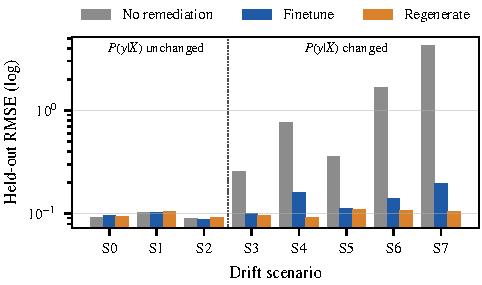
\includegraphics[width=\columnwidth]{figures/fig2_rmse.pdf}
\caption{Held-out RMSE by scenario and remediation action (logarithmic axis). Regenerate is the
stronger action wherever $P(y\mid X)$ has changed.}
\label{fig:rmse}
\end{figure}

\begin{figure}[t]
\centering
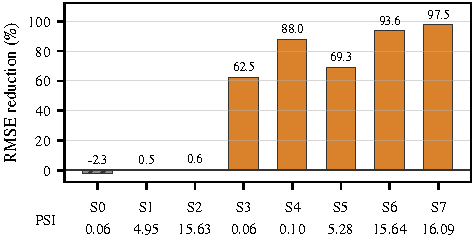
\includegraphics[width=\columnwidth]{figures/fig3_gain.pdf}
\caption{RMSE reduction by the better remediation arm per scenario, with
$\mathrm{PSI}_{\max}$ under each label. High PSI without concept drift (hatched) brings no
benefit; low PSI with concept drift (S3) brings a large one.}
\label{fig:gain}
\end{figure}

\subsection{PSI as a Severity Measure, Not a Trigger}
Fig.~\ref{fig:gain} shows the benefit of remediation per scenario with each scenario's
$\mathrm{PSI}_{\max}$. Scenario S2 records a PSI of 15.6, far above any conventional alert
threshold (0.25), yet remediation improves RMSE by only 0.63\,\%. Scenario S3 records 0.058,
below every conventional threshold, yet remediation improves RMSE by 62.49\,\%. This supports the
design of Fig.~\ref{fig:arch}: PSI is computed after a degradation has been reported and only
shapes the action (ruling out Finetune at $\mathrm{PSI}_{\max} \ge 0.5$). As an entry condition
it would have regenerated in S2, where nothing is gained, and stayed idle in S3, where the model
had become invalid; PSI must never trigger remediation on its own.

\begin{table}[t]
\centering
\caption{Deployment Gate Decisions (95\,\% Paired Bootstrap, 1000 Resamples)}
\label{tab:gate}
\footnotesize
\setlength{\tabcolsep}{2.4pt}
\resizebox{\columnwidth}{!}{%
\begin{tabular}{@{}lccccc@{}}
\toprule
Candidate & $\Delta$ & $\ell$ & $u$ & ${>}0$ (\%) & Verdict\\
\midrule
Exact least squares & $+0.00371$ & $+0.00037$ & $+0.00724$ & 98.9 & Deploy\\
SGD, other seed & $+0.00084$ & $+0.00034$ & $+0.00137$ & 100.0 & Deploy\\
Boosted stumps & $-0.00390$ & $-0.00956$ & $+0.00186$ & 10.0 & Reject\\
Copy of incumbent & $0.00000$ & $0.00000$ & $0.00000$ & 0.0 & Reject\\
Stale (baseline fit) & $-0.25842$ & $-0.27477$ & $-0.24131$ & 0.0 & Reject\\
Constant (mean) & $-0.11486$ & $-0.13934$ & $-0.09204$ & 0.0 & Reject\\
\bottomrule
\end{tabular}}

\vspace{2pt}
\parbox{\columnwidth}{\scriptsize $\Delta$: RMSE reduction against the incumbent (RMSE 0.1008);
${>}0$: share of resamples with $\Delta > 0$.}
\end{table}

\begin{figure}[t]
\centering
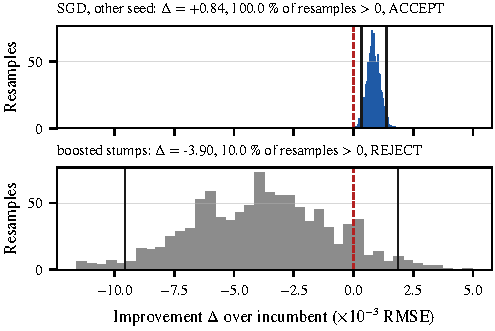
\includegraphics[width=\columnwidth]{figures/fig4_bootstrap.pdf}
\caption{Bootstrap distributions of the two decisive candidates. Solid lines: 95\,\% interval;
dashed line: $\delta = 0$.}
\label{fig:boot}
\end{figure}

\subsection{Deployment Gate Discrimination}
The gate of Eq.~\eqref{eq:gate} was exercised against six candidates of controlled quality. The
incumbent was itself fitted to a drifted window drawn with the parameters of S5, so all
differences are small;
against a stale incumbent every candidate would look excellent. Table~\ref{tab:gate} and
Fig.~\ref{fig:boot} report the outcome.

The second and third rows are decisive. A second SGD fit with another seed improves RMSE by only
0.00084, yet its entire interval lies above zero (100\,\% of resamples), so it is deployed. A
model of 300 boosted decision stumps has a point estimate four times larger in magnitude,
$-0.00390$, but its interval spans zero (10.0\,\% of resamples above it): it is not shown to
differ from the incumbent, and a lenient non-inferiority check on point estimates with a tolerance
of 0.004 would have promoted it. Under Eq.~\eqref{eq:gate} it is rejected and the incumbent is
retained. An identical copy ($\Delta = 0$ exactly) is rejected as well, because $\ell > 0$ is
strict.

\begin{figure}[t]
\centering
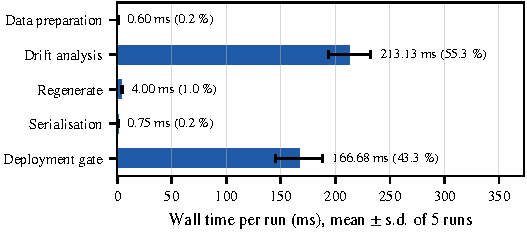
\includegraphics[width=\columnwidth]{figures/fig5_cost.pdf}
\caption{Wall time of one Regenerate run per stage (4 vCPU, Intel Xeon 2.1\,GHz).}
\label{fig:cost}
\end{figure}

\subsection{Computational Cost}
Fig.~\ref{fig:cost} gives the per-stage wall time of one Regenerate run, averaged over five
repetitions after a warm-up run, about 385\,ms in total. The shift analysis
($213.1 \pm 19.5$\,ms), which builds an Evidently report for the KS test and PSI of every
feature, and the gate ($166.7 \pm 21.9$\,ms) for its 1000 paired resamples dominate; the refit
itself takes 4\,ms on this small linear model. Both are negligible against the cadence of
readaptation requests; a similar model exchange skips training and the candidate gate.

\section{Limitations}
The similar model exchange path runs end to end, but its benefit was not quantified; that needs
a registry with many recorded versions and environments. The results use synthetic KPIs with
controlled covariate and concept shift and a linear model, not an operator trace, and the
remediation arms were executed with the scikit-learn engines only. Fine-tuning is a warm-start
continuation; parameter-efficient variants such as low-rank adaptation or partial layer freezing,
which limit catastrophic forgetting~\cite{kong2024overcoming}, are not implemented. A Rollback
decision of the Decision Engine does not itself re-promote a version. The framework treats a
reported degradation as drift; a degradation caused by conflicting xApps~\cite{adamczyk2023conflict,wadud2024qacm},
which calls for mitigation rather than retraining, is not diagnosed. Neither the LLM decision
agent nor the LLM-written engines and their repair loop were evaluated against a live LLM; they
were tested with a scripted LLM. Finally, registries, serving systems, and brokers were exercised
against emulators rather than live managed services.

\section{Conclusion and Future Work}
This paper presented an Agentic AI-based model regeneration framework for O-RAN that decides
when, and how, to readapt a degraded model.

The measured results support three claims. Regeneration is the stronger remediation action under
genuine concept drift, improving held-out RMSE by up to 97.5\,\%. Remediation brings no material
benefit under pure covariate shift even at a PSI of 15.6, which shows that PSI belongs after a
reported degradation as a severity measure, not before it as a trigger. And the deployment gate
rejects a candidate whose improvement interval includes zero even though its point estimate is
larger in magnitude than that of a deployed candidate.

Future work will measure the similar model exchange under realistic O-RAN shift, evaluate the LLM
decision agent and the LLM-written engines against live models and oracle choices on recorded
operator drift events, add parameter-efficient fine-tuning for deep-learning models, validate
candidates in a digital twin before the gate~\cite{masaracchia2023digital,zakihindi2026reference},
and diagnose xApp conflicts separately from drift.

\begin{thebibliography}{19}

\bibitem{polese2023understanding}
M.~Polese, L.~Bonati, S.~D'Oro, S.~Basagni, and T.~Melodia, ``Understanding O-RAN:
Architecture, interfaces, algorithms, security, and research challenges,'' \emph{IEEE Commun.
Surveys Tuts.}, vol.~25, no.~2, pp.~1376--1411, 2023.

\bibitem{ditzler2015learning}
G.~Ditzler, M.~Roveri, C.~Alippi, and R.~Polikar, ``Learning in nonstationary environments: A
survey,'' \emph{IEEE Comput. Intell. Mag.}, vol.~10, no.~4, pp.~12--25, 2015.

\bibitem{li2022rlops}
P.~Li \emph{et al.}, ``RLOps: Development life-cycle of reinforcement learning aided open RAN,''
\emph{IEEE Access}, vol.~10, pp.~113808--113826, 2022.

\bibitem{parraullauri2025reason}
J.~Parra-Ullauri \emph{et al.}, ``Lifecycle management of trustworthy AI models in 6G networks:
The REASON approach,'' \emph{IEEE Wireless Commun.}, vol.~32, no.~2, pp.~42--51, 2025.

\bibitem{mekrache2024intent}
A.~Mekrache, A.~Ksentini, and C.~Verikoukis, ``Intent-based management of next-generation
networks: An LLM-centric approach,'' \emph{IEEE Netw.}, vol.~38, no.~5, pp.~29--36, 2024.

\bibitem{bonati2021intelligence}
L.~Bonati, S.~D'Oro, M.~Polese, S.~Basagni, and T.~Melodia, ``Intelligence and learning in
O-RAN for data-driven NextG cellular networks,'' \emph{IEEE Commun. Mag.}, vol.~59, no.~10,
pp.~21--27, 2021.

\bibitem{polese2023coloran}
M.~Polese, L.~Bonati, S.~D'Oro, S.~Basagni, and T.~Melodia, ``ColO-RAN: Developing machine
learning-based xApps for open RAN closed-loop control on programmable experimental platforms,''
\emph{IEEE Trans. Mobile Comput.}, vol.~22, no.~10, pp.~5787--5800, 2023.

\bibitem{adamczyk2023conflict}
C.~Adamczyk and A.~Kliks, ``Conflict mitigation framework and conflict detection in O-RAN
near-RT RIC,'' \emph{IEEE Commun. Mag.}, vol.~61, no.~12, pp.~199--205, 2023.

\bibitem{wadud2024qacm}
A.~Wadud, F.~Golpayegani, and N.~Afraz, ``QACM: QoS-aware xApp conflict mitigation in open
RAN,'' \emph{IEEE Trans. Green Commun. Netw.}, vol.~8, no.~3, pp.~978--993, 2024.

\bibitem{zhou2025llm}
H.~Zhou \emph{et al.}, ``Large language model (LLM) for telecommunications: A comprehensive
survey on principles, key techniques, and opportunities,'' \emph{IEEE Commun. Surveys Tuts.},
vol.~27, no.~3, pp.~1955--2005, 2025.

\bibitem{leivadeas2023survey}
A.~Leivadeas and M.~Falkner, ``A survey on intent-based networking,'' \emph{IEEE Commun.
Surveys Tuts.}, vol.~25, no.~1, pp.~625--655, 2023.

\bibitem{masaracchia2023digital}
A.~Masaracchia, V.~Sharma, M.~Fahim, O.~A. Dobre, and T.~Q. Duong, ``Digital twin for open RAN:
Toward intelligent and resilient 6G radio access networks,'' \emph{IEEE Commun. Mag.}, vol.~61,
no.~11, pp.~112--118, 2023.

\bibitem{zakihindi2026reference}
A.~Zaki-Hindi \emph{et al.}, ``A reference functional architecture for network digital twins in
6G systems,'' \emph{IEEE Open J. Commun. Soc.}, vol.~7, pp.~2068--2101, 2026.

\bibitem{lacava2024programmable}
A.~Lacava \emph{et al.}, ``Programmable and customized intelligence for traffic steering in 5G
networks using open RAN architectures,'' \emph{IEEE Trans. Mobile Comput.}, vol.~23, no.~4,
pp.~2882--2897, 2024.

\bibitem{doro2022orchestran}
S.~D'Oro, L.~Bonati, M.~Polese, and T.~Melodia, ``OrchestRAN: Network automation through
orchestrated intelligence in the open RAN,'' in \emph{Proc. IEEE Conf. Comput. Commun.
(INFOCOM)}, 2022, pp.~270--279.

\bibitem{manias2022model}
D.~M. Manias, A.~Chouman, and A.~Shami, ``A model drift detection and adaptation framework for
5G core networks,'' in \emph{Proc. IEEE Int. Mediterranean Conf. Commun. Netw. (MeditCom)},
2022, pp.~197--202.

\bibitem{lu2019learning}
J.~Lu, A.~Liu, F.~Dong, F.~Gu, J.~Gama, and G.~Zhang, ``Learning under concept drift: A
review,'' \emph{IEEE Trans. Knowl. Data Eng.}, vol.~31, no.~12, pp.~2346--2363, 2019.

\bibitem{zoubir1998bootstrap}
A.~M. Zoubir and B.~Boashash, ``The bootstrap and its application in signal processing,''
\emph{IEEE Signal Process. Mag.}, vol.~15, no.~1, pp.~56--76, 1998.

\bibitem{kong2024overcoming}
Y.~Kong, L.~Liu, H.~Chen, J.~Kacprzyk, and D.~Tao, ``Overcoming catastrophic forgetting in
continual learning by exploring eigenvalues of Hessian matrix,'' \emph{IEEE Trans. Neural Netw.
Learn. Syst.}, vol.~35, no.~11, pp.~16196--16210, 2024.

\end{thebibliography}

\end{document}
